%%% Template by Mikhail Klassen, April 2013
%%% 
\documentclass[11pt,letterpaper]{article}
\newcommand{\workingDate}{\textsc{2019 $|$ April $|$ 21}}
\newcommand{\userName}{Jordan Sturtz}
\newcommand{\institution}{ Oregon State University}
\usepackage{researchdiary_png}
\usepackage{listings}
\usepackage{amsmath}

% To add your univerisity logo to the upper right, simply
% upload a file named "logo.png" using the files menu above.

\begin{document} \univlogo

\title{CS 475 - Parallel Programming}
{\Huge Project 2 Writeup}\\[5mm]

\begin{enumerate}
  \item \textbf{Estimated Volume = 28.69} 

    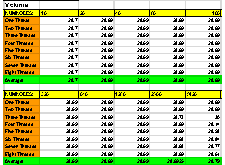
\includegraphics[width=\linewidth]{volume}
    
    The higher the NUMNODES, the more accurate the estimate of volume
    should be in principle since more subdivisions of the floor will better
    approximate our shape. Interestingly, however, we see a divergence
    in volume estimates for different threads when NUMNODES = 2560 or 5120. 
 
    When testing my code, I found no evidence of indeterministic code
    that might reveal race-condition failures: for any given NUMT and NUMNODES,
    the output was always the same. My hypothesis for the diverging estimates
    for the last two columns is this: higher values for NUMNODES and 
    higher threads involves more floating point additions. In addition, 
    these additions are adding smaller and smaller values since they subdivide
    the floor into smaller units. The floating point unit under the hood is
    probably rounding these smaller values in such a way as to produce
    inconsistent results. Given this inconsistency, I choose to use the earlier
    estimate for volume of 28.69.

  \item \textbf{Performance Summary} 

    I ran my tests on the oregonstate flip3 server. I wrote a shell script
    to execute my program with $NUMT = \{1 ... 8\}$ and with $NUMNODES = \{
      10, 20, 40, ... 5120 \}$.

    The performance results are shown in the following two tables:

    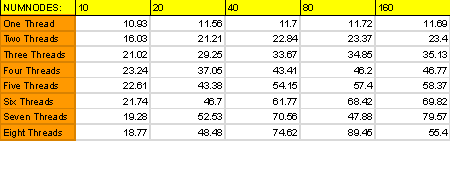
\includegraphics[width=\linewidth]{results2}
    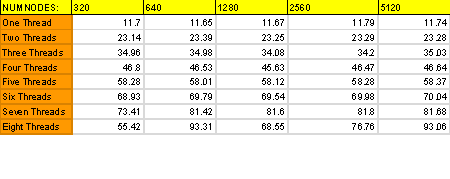
\includegraphics[width=\linewidth]{results3}

    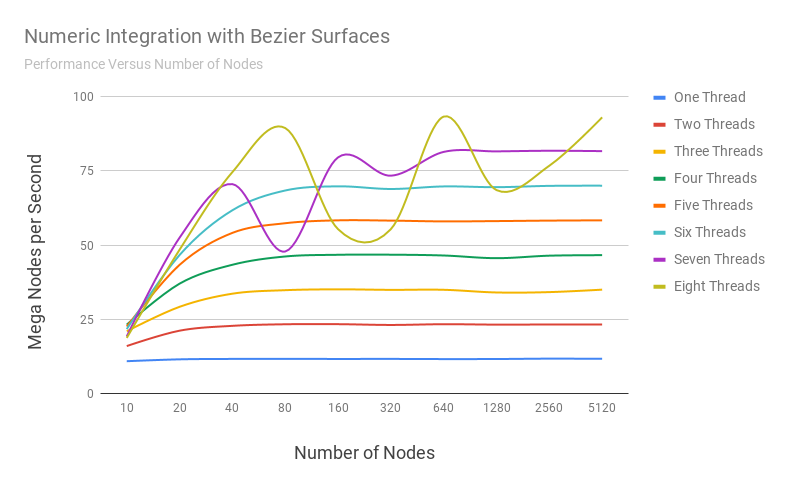
\includegraphics[width=\linewidth]{versusNodes}

    The only surprising result from this graph is that 
    there is high inconsistency in performance for execution with seven and 
    eight threads. My only current working hypothesis
    is that since the number of nodes is small, the higher thread executions
    create higher overhead in delegating fewer and fewer tasks. 
    However, I find this hypothesis unlikely since the actual
    work to delegate to each thread is equal to $NUMNODES^2 / NUMT$, which
    means that there are still many iterations to delegate to eight threads.
    Moreover, this hypothesis would explain only a diminishing return 
    and not, per se, the instability we find as the number of nodes increases
    for seven and eight threads. 

    
    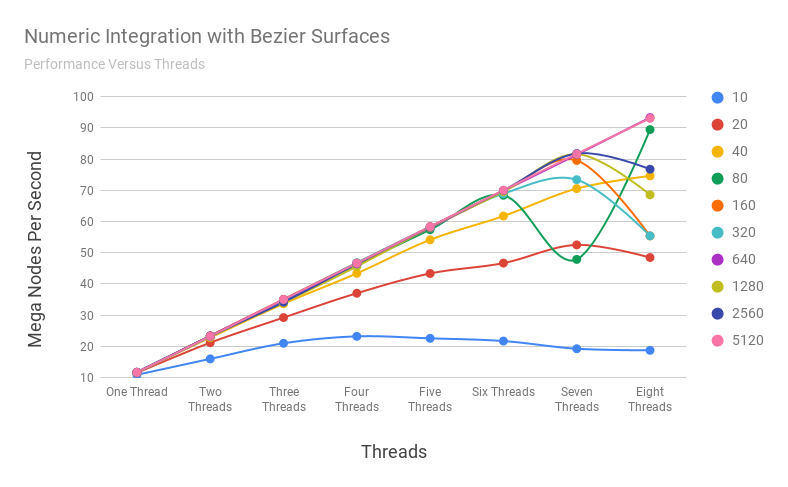
\includegraphics[width=\linewidth]{versusThreads}

    A noticable anomoly is the the execution with seven threads when 
    NUMNODES=80. This anomoly is probably due to a small fluctuation in
    server load during execution of my shell script, since further executions
    showed no particular drop in performance during that execution. Another
    interesting finding is that performance tends to more quickly plateau
    for smaller values of NUMNODES, which makes sense since the overhead for
    running a multithreaded program will tend against the minor performance
    gains in delegating a small number of tasks. 

  \item \textbf{Parallel Fraction} 
  
    My estimate for the parallel fraction is \textbf{0.997}. 
    I used the results from executing the code with eight
    threads and with 5120 number of nodes to estimate
    the parallel fraction. 
    
    The Inverse Amdahl's Law (i.e. solving Amdahl's for $P_f$) is 
    the following: 
    \begin{align*}
      F_p &= \frac{n}{n - 1}(1 - \frac{1}{S})
    \end{align*}

    where S is the speedup and n is the number of cores.  
    Let $S_1$ and $S_8$ be the speeds
    of the program executed with one thread and eight threads
    respectively. From my results, $S_1 = 11.74$ and $S_8 = 93.06$,
    so the speedup is $\frac{93.06}{11.74} = \mathbf{7.92}.$
    
    Subsituting into the Inverse Amdahl's Law:
    \begin{align*}
      F_p &= \frac{8}{8 - 1}(1 - \frac{1}{7.92})\\
      &= \mathbf{0.997}
    \end{align*}

  \item \textbf{Maximum Possible Speedup}

    The maximum possible speedup is: 
    \begin{align*}
      F_p &= \frac{1}{S_f}\\
    \end{align*}

    where $S_f$ is the sequential portion of the code. The sequential portion
    is the complement of the parallel fraction: 

    \begin{align*}
      F_p &= \frac{1}{1 - 0.997}\\
      &= \mathbf{333.33}
    \end{align*}



\end{enumerate}
\end{document}
